\begin{figure}[h]
  \centering
  \setlength{\unitlength}{\columnwidth}
  \begin{picture}(1,0.85)
    % figure labels
    \put(0.08,0.80){(a)}
    \put(0.48,0.80){(b)}
    \put(0.88,0.80){(c)}
    \put(0.48,0.40){(d)}
    % Components
    \put(0,0.65){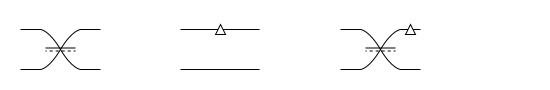
\includegraphics[width=\columnwidth]{figures/components}}
    % labels on components
    \put(0.18,0.70){\(r\)}
    \put(0.49,0.70){\(\phi\)}
    \put(0.80,0.70){\(r\)}
    \put(0.97,0.70){\(\phi\)}
    % Matrix labels of components
    \put(0,0.55){\(\begin{pmatrix}
      \sqrt{r} & \sqrt{1-r} \\
      \sqrt{1-r} & -\sqrt{r} \end{pmatrix}\)}
    \put(0.43,0.55){\(\begin{pmatrix}
      e^{i\phi} & 0 \\
      0 & 1 \end{pmatrix}\)}
    \put(0.65,0.55){\(\begin{pmatrix}
      e^{i\phi} \sqrt{r} & e^{i\phi} \sqrt{1-r} \\
      \sqrt{1-r} & -\sqrt{r} \end{pmatrix}\)}

    % Unitary/Reck scheme
    \put(0,0){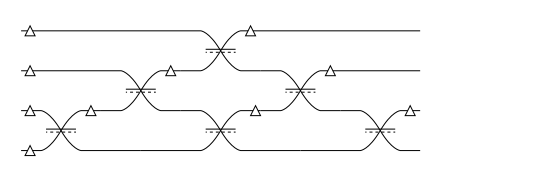
\includegraphics[width=\columnwidth]{figures/unitary}}
    % Beamsplitter labels
    \put(0.46,0.32){\(r_{4,1}\)}
    \put(0.27,0.22){\(r_{3,1}\)}
    \put(0.66,0.22){\(r_{4,2}\)}
    \put(0.07,0.12){\(r_{2,1}\)}
    \put(0.46,0.12){\(r_{3,2}\)}
    \put(0.85,0.12){\(r_{4,3}\)}
    % Phase shift labels
    \put(0.56,0.35){\(\phi_{4,1}\)}
    \put(0.37,0.25){\(\phi_{3,1}\)}
    \put(0.76,0.25){\(\phi_{4,2}\)}
    \put(0.17,0.15){\(\phi_{2,1}\)}
    \put(0.56,0.15){\(\phi_{3,2}\)}
    \put(0.95,0.15){\(\phi_{4,3}\)}
    % Input phase labels
    \put(0.0,0.35){\(\alpha_{4}\)}
    \put(0.0,0.25){\(\alpha_{3}\)}
    \put(0.0,0.15){\(\alpha_{2}\)}
    \put(0.0,0.05){\(\alpha_{1}\)}
  \end{picture}
  \caption{Linear-optical implementation of a unitary matrix.\\
    (a) and (b) are
    respectively a beamsplitter and phase shifter, and the matrix representation
    is indicated below. (c) is the combination of the two, and is the building
    block of the universal linear-optical circuit shown in (d). \\
    (d) shows a universal linear-optical circuit on four modes. If the
    parameters \(r_{ij}\)
    can be tuned between \(0\) and \(1\), and \(\phi_{i,j}\) and \(\alpha_i\)
    between \(0\) and \(2\pi\) then this configuration can realise any unitary
    operator on the input modes}
  \label{fig:unitary}
\end{figure}
